\documentclass[12pt]{report}
\usepackage{./sty/dissert}% style
\usepackage{comment}
\usepackage[acronym]{glossaries}
\usepackage{titlesec}
\usepackage{xcolor}
\usepackage{amsmath}
\usepackage{tikz}
\usepackage{float}
\usepackage{xcolor}
\usepackage{titlesec}
\definecolor{titulo}{RGB}{0,70,120}   % cor dos títulos (muda à vontade)

% Secção (3.4): maior, a cor, com uma linha por baixo
\titleformat{\section}
  {\Large\bfseries\color{titulo}}{\thesection}{0.8em}{\itshape}[{\color{titulo}\titlerule[0.8pt]}]
\titlespacing*{\section}{0pt}{3ex plus 1ex minus .2ex}{1.5ex plus .2ex}

% Subsecção (3.4.1): mais pequena, a negrito, sem cor nem linha
\titleformat{\subsection}
  {\large\bfseries}{\thesubsection}{0.8em}{}
\titlespacing*{\subsection}{0pt}{2.5ex plus 1ex minus .2ex}{1ex plus .2ex}

% Subsubsecção (3.4.1.1): tamanho do texto, itálico, sem número
\titleformat{\subsubsection}
  {\normalsize\bfseries\itshape}{}{0em}{}
  
\usetikzlibrary{calc,positioning}
\hypersetup{
    colorlinks,
    linkcolor={black!50!black},
    citecolor={black!50!black},
    urlcolor={black!80!black}
}
\titleformat{\chapter}{\LARGE}{\thechapter.}{20pt}{\LARGE\textbf}
\titlespacing*{\chapter}{0pt}{0pt}{20pt}
\renewcommand{\figurename}{Figura}
\titleformat*{\section}{\large\bfseries}
%
\makeglossaries%
 % ------------------- Document -----------------------------------------------------
\begin{document}
%\onehalfspacing
\pagenumbering{roman}
\newcommand\tab[1][1cm]{\hspace*{#1}}
% title page
\begin{titlepage}

\newcommand{\HRule}{\rule{\linewidth}{0.5mm}} % Defines a new command for the horizontal lines, change thickness here

\center % Center everything on the page
 %    LOGO SECTION

\FloatBarrier
\begin{figure}[ht!]
    \centering
    %\captionsetup{justification=centering,margin=2cm}
    
\includegraphics[width=0.4\textwidth]{img/logo.png}  
\end{figure}
\FloatBarrier
\vspace{0.5cm}

%    HEADING SECTIONS

{\LARGE Universidade do Minho}\\[0.5cm] % Name of your university/college
{\Large Escola de Engenharia}\\[0.5cm] % Name of your university/college
{\Large Mestrado em Engenharia Eletrónica Industrial e Computadores}\\[0.5cm] % Major heading such as course name

{\Large  Sistemas Autónomos Inteligentes}\\%[0.5cm] % Minor heading such as course title

%------------------------------------------------------------------------------------
%    TITLE SECTION1_Codigo

 {\large\emph{}}\\[1.5cm]
\HRule \\[0.3cm]

{\Huge  \bfseries \scshape Relatório de Cinemática}
\HRule \\[0.3cm]

%------------------------------------------------------------------------------------
%    AUTHOR SECTION

\vspace{1.50cm} %5mm vertical space
\Large{Autores:}\\
\vspace{0.20cm} %5mm vertical space
\begin{tabular}{ll}
    Fábio Alves & PG63877\\
    Lara Fernandes & PG63895\\
    Nádia Silva & PG63900\\
    Nuno Costa & PG63901\\
   
  \end{tabular}%
\\[1.3cm] % Your name

%------------------------------------------------------------------------------------
%    ACADEMIC ADVISORS SECTION

%\vspace{0.1mm} %5mm vertical space
Professora:\\
\vspace{0.20cm} %5mm vertical space
\begin{tabular}{ll}
    Estela Bicho\\

  \end{tabular}%
  \\[0.3cm] % Your name
%------------------------------------------------------------------------------------
%    DATE SECTION
%{\large \textsc{\today}}
%\vfill 
%\pagenumbering{arabic}
\end{titlepage}
%\pagenumbering{arabic}
\newpage
\newacronym{eeic}{EEIC}{Engenharia Eletrónica Industrial e de Computadores}
\newacronym{um}{UM}{Universidade do Minho}
%
% --------------Indices------------------
\renewcommand{\contentsname}{Índice}
\renewcommand{\listfigurename}{Lista de Figuras}
\renewcommand{\listtablename}{Lista de Tabelas}
\tableofcontents
\newpage
\listoffigures
\newpage
\listoftables
\newpage
%
\phantomsection%
%\addcontentsline{toc}{chapter}{Índice}
%\printglossary[type=\acronymtype,title=Lista de Abreviações]
\cleardoublepage%
%
% --------------TRABALHO------------------
\renewcommand\chaptername{Capítulo}
%----- INTRODUÇÃO -----------
\pagenumbering{arabic}
%
%

\chapter{Introdução}
\label{ch:intro}
O presente relatório foi desenvolvido no âmbito da unidade curricular de Sistemas Autónomos Inteligentes, do Mestrado em Engenharia Eletrónica Industrial e de Computadores da Universidade do Minho.

O trabalho centra-se no estudo e na implementação da cinemática do manipulador robótico myCobot~280, constituído por seis articulações rotativas. O objetivo consiste em determinar a posição do centro de preensão e a orientação da garra a partir das variáveis articulares, bem como calcular as configurações necessárias para alcançar diferentes posições no espaço de trabalho.

Para o desenvolvimento do projeto, foi utilizado o MATLAB, responsável pela implementação dos modelos cinemáticos e pelo controlo dos movimentos, e o CoppeliaSim, utilizado como ambiente de simulação para visualizar, testar e validar o comportamento do manipulador.

Ao longo do relatório são apresentados os fundamentos da cinemática direta e inversa, as respetivas formulações matemáticas, a implementação dos algoritmos em MATLAB e os resultados obtidos em ambiente de simulação.


\section{Fundamentos da cinemática}
\label{sec:fundamentos}

A cinemática de um manipulador robótico permite estabelecer a relação entre as variáveis articulares e a posição e orientação do \textit{end effector}. No caso do myCobot~280, constituído por seis articulações rotativas, esta análise divide-se em dois problemas fundamentais: a cinemática direta e a cinemática inversa.

A cinemática direta permite determinar a posição e orientação de um manipulador a partir dos ângulos das suas articulações. Por outro lado, a cinemática inversa permite determinar os ângulos articulares necessários para alcançar uma posição pretendida, considerando determinadas restrições de orientação.



\section{Enquadramento e objetivos}
\label{sec:enq-e-obj}

Os manipuladores robóticos desempenham um papel importante na automação industrial, sendo utilizados em tarefas que exigem precisão, repetibilidade e flexibilidade de movimentos. O seu funcionamento depende do conhecimento da geometria do manipulador e da relação entre as variáveis articulares e o posicionamento do \textit{end effector} no espaço de trabalho.

Neste contexto, o presente projeto centra-se no estudo do manipulador myCobot~280, recorrendo ao MATLAB para implementar os algoritmos cinemáticos e ao CoppeliaSim para simular e avaliar o comportamento do robô.

Os principais objetivos do trabalho são:

\begin{itemize}
    \item Desenvolver a formulação matemática da cinemática direta e inversa do manipulador;

    \item Implementar os modelos cinemáticos em MATLAB;

    \item Determinar a posição do centro de preensão e a direção da garra a partir dos ângulos articulares;

    \item Calcular as configurações articulares necessárias para alcançar posições pretendidas, considerando a inclinação da garra e os limites das juntas;

    \item Implementar movimentos no espaço das juntas e trajetórias no espaço cartesiano;

    \item Integrar o MATLAB com o CoppeliaSim para executar e visualizar os movimentos do manipulador;

    \item Explorar a utilização da visão artificial na identificação e localização de objetos;

    \item Validar os modelos implementados através da comparação entre os resultados calculados e os obtidos em simulação.
\end{itemize}


\setcounter{table}{0}
\setcounter{figure}{0}

\input{tex/Chap/2-Direct_Kin/DIR_KIN}
\setcounter{table}{0}
\setcounter{figure}{0}

\input{tex/Chap/3-Inverse_kin/INV_KIN}
\setcounter{table}{0}
\setcounter{figure}{0}

\chapter{Implementação em MATLAB}
\label{ch:matlab}

Neste subcapítulo, são apresentados os resultados obtidos após a junção do cenário de simulação do CoppeliaSim e a implementação da lógica da cinemática direta e inversa do manipulador robótico MyCobot280 em MATLAB. 

\section{Comunicação entre o MATLAB e o CoppeliaSim}
\label{sec:comunicacao}

A simulação corre em modo síncrono (\texttt{sim.setStepping(true)}): só avança um passo, de cerca de 50~ms, quando o MATLAB o pede. Assim, enquanto o MATLAB calcula, o simulador fica parado, e os resultados não dependem da velocidade do computador. A Tabela~\ref{tab:api} mostra as funções usadas no movimento do braço, das classes \texttt{mycobot\_interface} e \texttt{simulator\_interface} fornecidas.

\begin{table}[H]
  \centering
  \caption{Funções usadas para mover o braço e chamadas à API remota correspondentes.}
  \label{tab:api}
  \small
  \begin{tabular}{p{4.4cm}p{4.0cm}p{3.6cm}}
    \hline
    Função MATLAB & Chamada à API & Para quê \\[2pt]
    \hline
    \texttt{robot\_arm.set\_joints(q)} & \texttt{sim.setJoint}\allowbreak\texttt{TargetPosition} & enviar os ângulos pretendidos \\
    \texttt{robot\_arm.get\_joints()} & \texttt{sim.getJointPosition} & ler os ângulos das juntas \\
    \texttt{sim\_interface.}\allowbreak\texttt{step\_simulation()} & \texttt{sim.step} & avançar um passo \\
    \texttt{sim\_interface.}\allowbreak\texttt{get\_simulation\_time()} & \texttt{sim.getSimulationTime} & tempo de simulação \\
    \hline
  \end{tabular}
\end{table}

As leituras das juntas são o que os \textit{encoders} do braço real dariam. As posições reais dos objetos, que só o simulador conhece, são usadas apenas nos testes de diagnóstico, para medir os erros.

\section{Organização do código}
\label{sec:organizacao}
 
\begin{table}[H]
  \centering
  \caption{Funções do pacote \texttt{+movement} usadas nesta componente.}
  \label{tab:funcoes}
  \begin{tabular}{ll}
    \hline
    Função & O que faz \\
    \hline
    \texttt{direct\_kin} & cinemática direta (Capítulo~\ref{ch:dir_kin}) \\
    \texttt{ik\_2dof} & braço planar de 2 DOF, como na aula \\
    \texttt{inverse\_kin} & cinemática inversa (Capítulo~\ref{ch:inv_kin}) \\
    \texttt{move\_joints} & movimento suave no espaço das juntas \\
    \texttt{move\_linear} & movimento da garra em linha reta \\
    \texttt{go\_home} & regresso à pose inicial a partir de qualquer pose \\
    \texttt{plan\_vertical} & escolha de uma inclinação para toda uma descida \\
    \hline
  \end{tabular}
\end{table}

\section{Discussão}
\label{sec:disc}
 
\subsection{Validação do modelo}
 
O erro do modelo compara a posição calculada pela cinemática direta, com as juntas lidas no simulador, com a posição real do centro de preensão. Ficou entre 1,2 e 4,0~mm nos alvos testados, abaixo da tolerância de 5~mm, o que valida em conjunto a função \texttt{direct\_kin}, a conversão \texttt{world\_to\_base} e os comprimentos dos elos medidos no cenário. As diferenças que restam são pequenas e podem vir de os comprimentos medidos não coincidirem exatamente com a geometria do modelo do robô no CoppeliaSim e de o centro de preensão ser definido a partir de um ponto do modelo. Este erro não depende do movimento, pois só compara dois cálculos da mesma pose, e por isso mede a qualidade do modelo e não a do controlo.
 
\subsection{Erro de alcance e erro nas juntas}
 
O erro de alcance compara o ponto pedido com a posição real da garra, pelo que mistura dois efeitos: o erro do modelo e o facto de as juntas não chegarem exatamente aos ângulos pedidos. O erro nas juntas isola o segundo. Se o erro de alcance for semelhante ao erro do modelo e o erro nas juntas for pequeno, o movimento atinge o ponto pedido e o erro restante vem do modelo. Se o erro de alcance for maior, a diferença vem de as juntas ficarem ainda a caminho ou abaixo do ângulo pedido, por exemplo por efeito da gravidade ou do tempo de estabilização, de 2~s, ser curto para o movimento em causa.
\subsection{Alcance e inclinação da garra}
 
A cinemática inversa tenta primeiro a inclinação preferida, com a garra na vertical, e só se esta falhar inclina a garra. Com a implementação que usámos, para alvos a poucos centímetros da mesa, o alcance horizontal é de cerca de 27--28~cm do eixo da base com a garra na vertical e passa a cerca de 36--37~cm quando se permite inclinar a garra até $30^\circ$ da horizontal. Os alvos mais afastados da base são, por isso, os que exigem inclinar a garra, e são também os que deixam o braço quase esticado, onde pequenos erros nas juntas se traduzem em erros maiores de posição. Por outro lado, um alvo demasiado perto do eixo da base pode ser inalcançável, porque o desvio lateral $L_5$ impede a garra de chegar ao eixo de J1.
 
\subsection{Limitações}
 
O movimento \texttt{move\_joints} interpola as juntas, e não a posição da garra, pelo que a trajetória do \textit{end-effector} entre dois pontos não é uma reta; passa pela pose inicial para evitar a mesa, mas não é uma trajetória planeada no espaço cartesiano. Quando é preciso um movimento em linha reta, usa-se \texttt{move\_linear}, que resolve a cinemática inversa a cada passo. Além disso, os resultados são de simulação e usam as posições reais dos objetos, que só o simulador conhece, apenas para definir os alvos e medir os erros; no braço real, os alvos viriam da câmara e não existiria o erro do modelo medido desta forma.
 

\section{Cinemática direta}
\label{sec:cin_dir}

A função \texttt{direct\_kin} serve para implementar a Equação~\eqref{eq:dk_final}, seguindo a mesma ordem de dedução utilizada anteriormente.

\begin{lstlisting}[language=Matlab, caption={Função \texttt{direct\_kin}}, label={lst:dir_kin}]
function [tip, approach] = direct_kin(q, Links)
    q = q(:)';
    if numel(q) == 4
        q = [q 0 0];                % bloquear J5 e J6 
    end
    L = Links;
    D = L(6) + L(7);    

    thetaA = q(2) + pi/2;           % elo L2 (J2 -> J3)
    thetaB = thetaA + q(3);         % elo L3 (J3 -> J4)
    thetaC = thetaB + q(4);         % elo L4 (J4 -> J5)
    alpha  = thetaC - pi/2;         % garra: perpendicular a L4 (-90 graus = para baixo)

    % J2 (ombro)
    d = 0;                          h = L(1);
    % J3 (cotovelo)
    d = d + L(2)*cos(thetaA);       h = h + L(2)*sin(thetaA);
    % J4 (pulso)
    d = d + L(3)*cos(thetaB);       h = h + L(3)*sin(thetaB);
    % J5
    d = d + L(4)*cos(thetaC);       h = h + L(4)*sin(thetaC);
    % centro de preensao
    d = d + D*cos(q(5))*cos(alpha); h = h + D*cos(q(5))*sin(alpha);
    l = L(5) - D*sin(q(5));        

    x = l*cos(q(1)) + d*cos(q(1) + pi/2);  % = l*cos(q1) - d*sin(q1)
    y = l*sin(q(1)) + d*sin(q(1) + pi/2);  % = l*sin(q1) + d*cos(q1)
    z = h;
    tip = [x; y; z];

    aL = -sin(q(5));                % componente lateral
    aD =  cos(q(5))*cos(alpha);     % componente em frente
    aH =  cos(q(5))*sin(alpha);     % componente para cima
    approach = [aL*cos(q(1)) + aD*cos(q(1) + pi/2);
                aL*sin(q(1)) + aD*sin(q(1) + pi/2);
                aH];
end
\end{lstlisting}

\begin{table}[H]
  \centering
  \caption{Entradas e saídas de \texttt{direct\_kin}.}
  \label{tab:direct_io}
  \begin{tabular}{ll}
    \toprule
    Argumento & Significado \\
    \midrule
    \multicolumn{2}{l}{\textit{Entradas}} \\
    \texttt{q}     & ângulos das juntas [rad], $1\times4$ ou $1\times6$ \\
    \texttt{Links} & os sete comprimentos da Tabela~\ref{tab:elos} [m] \\
    \midrule
    \multicolumn{2}{l}{\textit{Saídas}} \\
    \texttt{tip}      & posição $3\times1$ do centro de preensão, referencial da base [m] \\
    \texttt{approach} & vetor unitário da direção da garra \\
    \bottomrule
  \end{tabular}
\end{table}

Esta função é utilizada em vários pontos da execução para identificar a posição da garra a partir das leituras das juntas

\section{Cinemática inversa}
\label{sec:cin_inv}

A função \texttt{inverse\_kin} implementa a formulação matemática da cinemática inversa apresentada no Capítulo~\ref{ch:inv_kin}, permitindo determinar os ângulos articulares necessários para alcançar uma posição pretendida do centro de preensão.

A resolução é realizada com o auxílio das funções \texttt{ik\_2dof} e \texttt{solve\_pitch}. A primeira resolve o problema geométrico de um manipulador planar de dois graus de liberdade, enquanto a segunda determina os ângulos das juntas J1 a J4 para uma inclinação específica da garra, verificando as restrições de alcance e os limites articulares.

A função principal começa por calcular a distância frontal e a altura relativamente ao ombro. Seguidamente, procura uma inclinação válida para a garra, começando pela orientação preferencial de $90^\circ$ e testando, quando necessário, inclinações alternativas em incrementos de $5^\circ$.

Quando é encontrada uma solução válida numa inclinação diferente da preferencial, é realizado um refinamento através do método da bisseção. Por fim, é calculada a rotação da junta J6, caso tenha sido fornecida a orientação do objeto e a inclinação da garra satisfaça a condição estabelecida.

A implementação da função principal encontra-se apresentada na Listagem~\ref{lst:inv_kin}.

\begin{lstlisting}[
    language=Matlab,
    caption={Implementação da função inverse\_kin.},
    label={lst:inv_kin}
]
function [armJoints, isReachable, pitchUsed] = ...
    inverse_kin(x, y, z, Links, qMin, qMax, ...
                objYaw, prefPitch, family, fixedPitch)

    % Valores por defeito
    if nargin < 5 || isempty(qMin)
        qMin = deg2rad([-165 -165 -165 -165 -165 -175]);
    end
    if nargin < 6 || isempty(qMax)
        qMax = deg2rad([165 165 165 165 165 175]);
    end
    if nargin < 7
        objYaw = [];
    end
    if nargin < 8 || isempty(prefPitch)
        prefPitch = pi/2;
    end
    if nargin < 9 || isempty(family)
        family = 'up';
    end
    if nargin < 10 || isempty(fixedPitch)
        fixedPitch = false;
    end

    L = Links;
    D = L(6) + L(7);

    armJoints = zeros(1,6);
    isReachable = false;
    pitchUsed = NaN;

    % Plano horizontal
    r = hypot(x,y);
    if r <= L(5)
        return;
    end

    dFwd = sqrt(r^2-L(5)^2);
    hJ2 = z-L(1);

    % Restricoes
    ELBOW_MAX = deg2rad(140);
    PITCH_MAX = deg2rad(135);
    PITCH_MIN = deg2rad(30);
    STEP = deg2rad(5);

    if ~strcmp(family,'down')
        family = 'up';
    end

    if fixedPitch
        dList = 0;
    else
        dList = 0:STEP:(PITCH_MAX-PITCH_MIN);
    end

    % Procurar inclinacao valida
    for d = dList
        if d == 0
            cands = prefPitch;
        else
            cands = [prefPitch+d, prefPitch-d];
        end

        for psi = cands
            if ~fixedPitch && ...
                    (psi > PITCH_MAX || psi < PITCH_MIN)
                continue;
            end

            best = solve_pitch(psi,x,y,dFwd,hJ2, ...
                L,D,qMin,qMax,ELBOW_MAX,family);

            if isempty(best)
                continue;
            end

            % Refinamento por bissecao
            if d > 0
                good = psi;
                bad = psi-sign(psi-prefPitch)*STEP;

                for it = 1:15
                    mid = (good+bad)/2;
                    qm = solve_pitch(mid,x,y,dFwd,hJ2, ...
                        L,D,qMin,qMax,ELBOW_MAX,family);

                    if isempty(qm)
                        bad = mid;
                    else
                        good = mid;
                        best = qm;
                    end
                end
                psi = good;
            end

            % Orientacao da junta J6
            q6 = 0;
            if ~isempty(objYaw) && psi > deg2rad(45)
                q6 = mod(best(1)-objYaw+pi/4,pi/2)-pi/4;
            end

            armJoints = [best 0 q6];
            isReachable = true;
            pitchUsed = psi;
            return;
        end
    end
end
\end{lstlisting}

A função devolve os seis ângulos articulares, um indicador de existência de solução e a inclinação efetivamente utilizada. Quando não é encontrada uma configuração válida, o indicador \texttt{isReachable} permanece falso.

O argumento \texttt{fixedPitch} permite desativar a procura automática de inclinações alternativas, sendo utilizado, por exemplo, em movimentos verticais nos quais se pretende manter a mesma orientação da garra ao longo da trajetória.

As entradas e saídas da função encontram-se resumidas na Tabela~\ref{tab:inverse_io}.

\begin{table}[H]
    \centering
    \caption{Entradas e saídas da função \texttt{inverse\_kin}.}
    \label{tab:inverse_io}
    \small
    \begin{tabular}{lp{8.5cm}}
        \hline
        Argumento & Significado \\
        \hline
        \multicolumn{2}{l}{\textit{Entradas}} \\
        \texttt{x, y, z} & Posição pretendida no referencial da base [m] \\
        \texttt{Links} & Parâmetros geométricos do manipulador [m] \\
        \texttt{qMin, qMax} & Limites articulares [rad] \\
        \texttt{objYaw} & Orientação do objeto em torno de $z$, opcional [rad] \\
        \texttt{prefPitch} & Inclinação preferencial da garra, opcional [rad] \\
        \texttt{family} & Configuração \texttt{'up'} ou \texttt{'down'}, opcional \\
        \texttt{fixedPitch} & Utilização exclusiva da inclinação indicada, opcional \\
        \hline
        \multicolumn{2}{l}{\textit{Saídas}} \\
        \texttt{armJoints} & Vetor $[q_1\ q_2\ q_3\ q_4\ q_5\ q_6]$ [rad] \\
        \texttt{isReachable} & Indicador de existência de solução válida \\
        \texttt{pitchUsed} & Inclinação efetivamente utilizada [rad] \\
        \hline
    \end{tabular}
\end{table}

\subsection{Funções auxiliares da cinemática inversa}

A função \texttt{ik\_2dof} resolve a cinemática inversa do braço planar formado pelos elos $L_2$ e $L_3$, através da lei dos cossenos. A implementação permite selecionar a configuração com o cotovelo para cima ou para baixo, conforme descrito na Secção~\ref{sec:ik_lateral}.

Por sua vez, a função \texttt{solve\_pitch} recebe uma inclinação $\psi$ previamente definida, calcula a posição do pulso J4 e utiliza \texttt{ik\_2dof} para determinar os ângulos das juntas J2 e J3. Seguidamente, determina J1 e J4 e verifica se a configuração obtida respeita os limites articulares, a flexão máxima do cotovelo e as restrições de altura das juntas.

As implementações destas funções encontram-se nas Listagens~\ref{lst:ik2dof} e~\ref{lst:solvepitch}.

\begin{lstlisting}[
    language=Matlab,
    caption={Implementação da função ik\_2dof.},
    label={lst:ik2dof}
]
function [theta1, theta2, isReachable] = ...
    ik_2dof(xd, yd, LA, LB, solution_type)

    theta1 = NaN;
    theta2 = NaN;
    isReachable = false;

    r = sqrt(xd^2+yd^2);
    alpha1 = atan2(yd,xd);

    arg1 = (LA^2+r^2-LB^2)/(2*LA*r);
    arg2 = (LA^2+LB^2-r^2)/(2*LA*LB);

    if r == 0 || abs(arg1) > 1 || abs(arg2) > 1
        return;
    end

    beta1 = acos(arg1);
    beta2 = acos(arg2);

    if strcmp(solution_type,'down')
        theta1 = alpha1-beta1;
        theta2 = pi-beta2;
    else
        theta1 = alpha1+beta1;
        theta2 = -(pi-beta2);
    end

    isReachable = true;
end
\end{lstlisting}

\begin{lstlisting}[
    language=Matlab,
    caption={Implementação da função solve\_pitch.},
    label={lst:solvepitch}
]
function q = solve_pitch(psi,x,y,dFwd,hJ2, ...
    L,D,qMin,qMax,elbowMax,family)

    wrap = @(t) atan2(sin(t),cos(t));
    q = [];

    % Angulo da base
    q1 = atan2(y,x)-atan2(dFwd,L(5));

    % Posicao do pulso
    alpha3 = -psi;
    x3d = dFwd-D*cos(alpha3) ...
        -L(4)*cos(alpha3+pi/2);
    y3d = hJ2-D*sin(alpha3) ...
        -L(4)*sin(alpha3+pi/2);

    % Braco planar de dois elos
    [theta1,theta2,ok] = movement.ik_2dof( ...
        x3d,y3d,L(2),L(3),family);

    if ~ok
        return;
    end

    % Angulo da junta J4
    theta3 = (alpha3+pi/2)-theta1-theta2;

    % Angulos articulares
    q = wrap([q1,theta1-pi/2,theta2,theta3]);

    % Alturas das juntas
    zElbow = L(1)+L(2)*cos(q(2));
    zJ4 = zElbow+L(3)*cos(q(2)+q(3));
    zJ5 = zJ4+L(4)*cos(q(2)+q(3)+q(4));

    % Validacao da configuracao
    if any(q < qMin(1:4)) || ...
            any(q > qMax(1:4)) || ...
            abs(q(3)) > elbowMax || ...
            min([zElbow zJ4 zJ5]) <= 0
        q = [];
    end
end
\end{lstlisting}

As entradas e saídas das duas funções auxiliares encontram-se apresentadas nas Tabelas~\ref{tab:ik2dof_io} e~\ref{tab:solvepitch_io}.

\begin{table}[H]
    \centering
    \caption{Entradas e saídas da função \texttt{ik\_2dof}.}
    \label{tab:ik2dof_io}
    \small
    \begin{tabular}{lp{8cm}}
        \toprule
        Argumento & Significado \\
        \midrule
        \multicolumn{2}{l}{\textit{Entradas}} \\
        \texttt{xd, yd} & Coordenadas do pulso relativamente ao ombro [m] \\
        \texttt{LA, LB} & Comprimentos dos dois elos [m] \\
        \texttt{solution\_type} & Configuração \texttt{'up'} ou \texttt{'down'} \\
        \midrule
        \multicolumn{2}{l}{\textit{Saídas}} \\
        \texttt{theta1} & Orientação absoluta do primeiro elo [rad] \\
        \texttt{theta2} & Rotação do segundo elo relativamente ao primeiro [rad] \\
        \texttt{isReachable} & Indicador de solução geométrica válida \\
        \bottomrule
    \end{tabular}
\end{table}

\begin{table}[H]
    \centering
    \caption{Entradas e saídas da função \texttt{solve\_pitch}.}
    \label{tab:solvepitch_io}
    \small
    \begin{tabular}{lp{8cm}}
        \toprule
        Argumento & Significado \\
        \midrule
        \multicolumn{2}{l}{\textit{Entradas}} \\
        \texttt{psi} & Inclinação definida para a garra [rad] \\
        \texttt{x, y} & Coordenadas horizontais do alvo [m] \\
        \texttt{dFwd, hJ2} & Distância frontal e altura relativa ao ombro [m] \\
        \texttt{L, D} & Parâmetros geométricos do manipulador [m] \\
        \texttt{qMin, qMax} & Limites articulares [rad] \\
        \texttt{elbowMax} & Flexão máxima admitida para o cotovelo [rad] \\
        \texttt{family} & Configuração \texttt{'up'} ou \texttt{'down'} \\
        \midrule
        \multicolumn{2}{l}{\textit{Saída}} \\
        \texttt{q} & Vetor $[q_1\ q_2\ q_3\ q_4]$ [rad] ou vazio \\
        \bottomrule
    \end{tabular}
\end{table}

Deste modo, a implementação separa a procura de uma inclinação válida da resolução geométrica para uma inclinação específica, permitindo reutilizar os cálculos cinemáticos em diferentes procedimentos de movimento.

A função \texttt{inverse\_kin} é utilizada tanto no posicionamento do manipulador como no planeamento de trajetórias, sendo chamada repetidamente quando é necessário determinar configurações articulares para diferentes pontos do espaço de trabalho.


\section{Movimento até uma posição alvo}
\label{sec:imp_move}

O movimento do manipulador até uma posição pretendida envolve a transformação das coordenadas do alvo, o cálculo da configuração articular e a execução do movimento através das funções desenvolvidas em MATLAB.

Quando a posição do alvo é fornecida no referencial do mundo do CoppeliaSim, o procedimento pode ser dividido nas seguintes etapas:

\begin{enumerate}
    \item \textbf{Transformação de coordenadas:}
    a posição pretendida $(X_{\mathrm{target}},Y_{\mathrm{target}},Z_{\mathrm{target}})$ é convertida para o referencial da base do manipulador através da função \texttt{aux.world\_to\_base}, considerando a translação e a rotação entre os dois referenciais;

    \item \textbf{Cálculo da configuração articular:}
    a função \texttt{inverse\_kin} determina os ângulos necessários para alcançar a posição pretendida, respeitando as restrições geométricas e articulares definidas. Caso não exista uma solução válida, o movimento pode ser rejeitado antes da sua execução;

    \item \textbf{Execução do movimento:}
    após determinar uma configuração válida, o manipulador pode ser deslocado através da função \texttt{move\_joints}, que realiza a interpolação dos ângulos articulares, ou da função \texttt{move\_linear}, utilizada quando se pretende seguir uma trajetória aproximadamente retilínea no espaço cartesiano;

    \item \textbf{Verificação do posicionamento:}
    os ângulos articulares obtidos durante a execução podem ser utilizados pela função \texttt{direct\_kin} para calcular a posição do centro de preensão e avaliar a diferença relativamente à posição pretendida.
\end{enumerate}

\subsection{Movimento no espaço das juntas}

A função \texttt{move\_joints} permite deslocar o manipulador entre duas configurações articulares, garantindo uma evolução suave dos ângulos das juntas.

Em vez de enviar diretamente os ângulos finais, a função calcula, em cada passo de simulação, uma configuração intermédia entre a configuração inicial e a pretendida. Todas as juntas iniciam e terminam o movimento ao mesmo tempo, independentemente da amplitude da rotação de cada uma.

A evolução entre as duas configurações segue um perfil suave, em forma de S: as juntas arrancam devagar, aceleram até ao meio do movimento e abrandam até parar na posição pretendida. Desta forma, o movimento começa e termina com velocidade nula, evitando alterações bruscas da velocidade e solavancos no manipulador.

A duração do movimento é definida pela junta que tem de rodar mais. Esta duração é calculada de modo a que a velocidade dessa junta nunca ultrapasse a velocidade máxima pretendida, de $30^\circ$/s por defeito. As restantes juntas, como rodam menos no mesmo tempo, movem-se mais devagar.

A execução é realizada de forma sincronizada, sendo enviadas configurações articulares intermédias ao manipulador em cada passo de simulação.

No final, a função verifica se todas as juntas se encontram a menos de $1^\circ$ dos respetivos valores pretendidos.
\subsection{Movimentos em linha reta}

Para movimentos de aproximação a objetos, nomeadamente durante a descida da garra até uma peça, é utilizada a função \texttt{move\_linear}.

Ao contrário do movimento no espaço das juntas, esta função faz evoluir um ponto de referência ao longo da direção que une a posição atual do centro de preensão à posição pretendida.

Em cada passo de simulação, o programa atualiza a velocidade do ponto de referência, respeitando a velocidade máxima definida e a aceleração configurada através do parâmetro \texttt{cfg.ACC}.

A velocidade é aumentada gradualmente e reduzida à medida que o ponto se aproxima do destino, de forma a evitar uma paragem brusca.

Para cada posição intermédia, a função \texttt{inverse\_kin} calcula os ângulos articulares correspondentes, que são enviados ao manipulador.

Após o ponto de referência atingir o destino, o programa compara a posição pretendida com a posição calculada pela cinemática direta a partir dos ângulos efetivamente lidos.

Quando necessário, é aplicada uma correção progressiva ao ponto de referência para compensar diferenças de posicionamento, incluindo os efeitos associados à gravidade.

O movimento é considerado concluído com sucesso quando o erro de posicionamento é inferior a $3$ mm, dentro das condições de execução estabelecidas.

\subsection{Planeamento de movimentos verticais}

Antes de executar determinados movimentos verticais, a função \texttt{plan\_vertical} seleciona uma inclinação fixa da garra que permita percorrer toda a trajetória.

Este procedimento é particularmente importante durante a aproximação a objetos situados perto da base do manipulador, onde pequenas alterações de posição podem exigir variações significativas dos ângulos articulares.

O algoritmo testa diferentes inclinações, começando pela orientação vertical para baixo, correspondente a $\psi=90^\circ$.

Para cada inclinação candidata, são verificadas sucessivamente as posições ao longo da trajetória vertical, em intervalos de $2$ mm.

Uma inclinação apenas é aceite quando são satisfeitas as seguintes condições:

\begin{itemize}
    \item Existe uma solução válida de cinemática inversa para todos os pontos da trajetória;

    \item A variação de cada uma das juntas J1 a J4 entre posições consecutivas não ultrapassa $5^\circ$;

    \item Quando a verificação de colisões está ativada, as configurações articulares não provocam colisões do manipulador consigo próprio.
\end{itemize}

Durante esta verificação, é utilizada a configuração com o cotovelo para cima, sendo mantida a mesma inclinação da garra ao longo de todo o movimento.

Esta abordagem reduz a possibilidade de alterações abruptas das configurações articulares durante a descida.

A Figura~\ref{fig:move} apresenta uma representação esquemática da sequência de aproximação a uma peça.

\begin{figure}[htbp]
    \centering
    % Sequência do movimento até uma peça, vista lateral (esboço, sem escala)
\begin{tikzpicture}[scale=1.2, >=stealth,
    elo/.style={line width=2pt, line cap=round},
    junta/.style={circle, draw, fill=white, line width=0.9pt, inner sep=1.6pt},
    pt/.style={circle, fill, inner sep=1.5pt},
    every node/.style={font=\footnotesize}]

  % mesa e base
  \fill[pattern=north east lines, pattern color=gray!60] (-1.2,-0.25) rectangle (10.2,0);
  \draw[thick] (-1.2,0) -- (10.2,0) node[below left=2pt and 0pt] {mesa};
  \fill[gray!30] (-0.45,0) rectangle (0.45,0.5);
  \draw (-0.45,0) rectangle (0.45,0.5);
  % braço na pose inicial (esboço)
  \coordinate (J2) at (0,1.6);
  \draw[elo, gray!70] (0,0.5) -- (J2) -- (0.3,3.3) -- (1.6,4.1);
  \node[junta] at (J2) {}; \node[junta] at (0.3,3.3) {};
  % peça
  \fill[red!65] (6.3,0) rectangle (7.1,0.8);
  \draw (6.3,0) rectangle (7.1,0.8);

  \coordinate (P0) at (1.6,4.1);
  \coordinate (P1) at (6.7,3.0);
  \coordinate (P2) at (6.7,1.4);

  % 1: move_joints (trajetória curva da garra)
  \draw[->, blue!70!black, line width=1.1pt, dashed] (P0) .. controls (3.6,5.2) and (5.8,4.4) .. (P1);
  \node[blue!70!black, align=center] at (3.9,5.35) {\textbf{1.} \texttt{move\_joints}};
  % 2: move_linear (descida vertical)
  \draw[->, orange!85!black, line width=1.3pt] (P1) -- (P2);
  \foreach \h in {2.8,2.6,...,1.5} \draw[orange!85!black] (6.6,\h) -- (6.8,\h);
  \node[orange!85!black, align=left, anchor=west] at (7.7,2.4) {\textbf{2.} \texttt{move\_linear}\\descida em linha reta,\\uma só inclinação\\(\texttt{plan\_vertical},\\de 2 em 2 mm)};
  % 3: subida e go_home
  \draw[->, green!45!black, line width=1.1pt, dotted] (6.2,1.5) -- (6.2,2.9) .. controls (5.0,4.0) and (3.0,4.6) .. (1.8,4.25);
  \node[green!45!black, align=center] at (3.5,3.1) {\textbf{3.} \texttt{go\_home}: sobe na\\vertical e regressa};

  \node[pt] at (P0) {}; \node[above left=1pt and 0pt] at (P0) {pose inicial};
  \node[pt] at (P1) {}; \node[above right=5pt and 2pt] at (P1) {aproximação};
  \node[pt] at (P2) {};
  \draw[<->, gray!70!black, thin] (7.35,0) -- (7.35,1.4) node[midway, right, black] {2 cm};
  \draw[gray!70!black, thin, dashed] (6.7,1.4) -- (7.45,1.4);
\end{tikzpicture}
    \caption{Representação esquemática da sequência de movimento até uma peça, numa vista lateral e sem escala.}
    \label{fig:move}
\end{figure}

\subsection{Regresso à pose inicial}

A função \texttt{go\_home} permite deslocar o manipulador para uma configuração inicial previamente definida, independentemente da posição articular de partida, desde que o movimento seja realizável.

O procedimento começa pela abertura da garra e pela leitura dos ângulos articulares atuais.

Através da função \texttt{direct\_kin}, é determinada a posição do centro de preensão. Caso a sua altura seja inferior ao valor de segurança definido, de $0{,}15$ m relativamente à base, o algoritmo procura realizar uma subida gradual antes do regresso à configuração inicial.

Durante esta subida, são calculadas sucessivamente novas configurações articulares através da função \texttt{inverse\_kin}, procurando manter a inclinação inicial da garra.

Se não for possível encontrar uma configuração válida ou se forem detetadas variações articulares excessivas, a subida é interrompida e o programa avança para a etapa seguinte.

Posteriormente, a função \texttt{move\_joints} é utilizada para executar o movimento suave até à configuração inicial.

Por fim, os ângulos articulares são novamente lidos, sendo o regresso considerado bem-sucedido quando todas as juntas apresentam um desvio inferior a $1^\circ$ relativamente aos valores pretendidos.

Este procedimento baseia-se nas leituras articulares, permitindo utilizar a mesma lógica de controlo com a interface do manipulador simulado ou com uma interface compatível de um braço físico.

\setcounter{table}{0}
\setcounter{figure}{0}

\chapter{Resultados e discussão}
\label{ch:res-e-disc}

Neste capítulo, são apresentados os resultados matemáticos das equações da cinemática direta e inversa, bem como os resultados da implementação dos modelos de cinemática do myCobot~280 em MATLAB e da sua validação no CoppeliaSim.

Serão analisados os exemplos de posicionamento, os erros obtidos nos testes e as principais limitações do sistema.

\section{Resultados}
\label{sec:result}

\subsection{Demonstração no simulador}
\label{sec:demo_sim}

Para demonstrar o movimento \textit{move end-effector to target position} para diferentes posições alvo, o manipulador foi levado, no CoppeliaSim, até cada uma das peças detetadas pela câmara na mesa. Para cada alvo, a \texttt{inverse\_kin} calcula os ângulos das juntas, a \texttt{move\_joints} leva o braço até por cima da peça e a \texttt{move\_linear} desce na vertical até 2~cm acima da mesa. Mediram-se três erros:

\begin{itemize}
    \item \textbf{modelo}: distância entre a posição dada pela \texttt{direct\_kin}, com as juntas lidas, e a posição real do centro de preensão no simulador;
    \item \textbf{alcance}: distância entre o ponto pedido e a posição real do centro de preensão;
    \item \textbf{juntas}: maior diferença entre os ângulos calculados e os ângulos lidos.
\end{itemize}

\begin{table}[H]
  \centering
  \caption{Resultados do movimento até diferentes posições alvo no simulador.}
  \label{tab:demo_sim}
  \resizebox{\textwidth}{!}{%
  \begin{tabular}{lcccccc}
    \toprule
    Peça & Pedido $(x, y, z)$ & Alcançado $(x, y, z)$ & $\psi$ & Modelo [mm] & Alcance [mm] & Juntas \\
    \midrule
    vermelho 1 & $(66{,}1;\ 199{,}9;\ -10{,}0)$ & $(65{,}7;\ 196{,}7;\ -11{,}3)$ & $90^\circ$ & 1,5 & 3,5 & $0{,}8^\circ$ \\
    vermelho 2 & $(-111{,}0;\ -37{,}2;\ -10{,}0)$ & $(-111{,}0;\ -38{,}2;\ -10{,}7)$ & $110^\circ$ & 2,3 & 1,3 & $0{,}4^\circ$ \\
    laranja & $(-107{,}9;\ 224{,}1;\ -10{,}0)$ & $(-106{,}0;\ 221{,}2;\ -12{,}4)$ & $90^\circ$ & 2,3 & 4,2 & $1{,}2^\circ$ \\
    amarelo & $(-33{,}5;\ 149{,}7;\ -10{,}0)$ & $(-33{,}0;\ 148{,}0;\ -9{,}7)$ & $95^\circ$ & 1,2 & 1,8 & $0{,}6^\circ$ \\
    verde & $(-129{,}4;\ 54{,}3;\ -10{,}0)$ & $(-128{,}7;\ 53{,}9;\ -10{,}0)$ & $100^\circ$ & 1,2 & 0,8 & $0{,}5^\circ$ \\
    azul & $(-147{,}3;\ 33{,}2;\ -10{,}0)$ & $(-145{,}6;\ 33{,}0;\ -9{,}8)$ & $95^\circ$ & 1,2 & 1,7 & $0{,}6^\circ$ \\
    rosa & $(16{,}3;\ 274{,}4;\ -10{,}0)$ & $(16{,}7;\ 269{,}6;\ -13{,}5)$ & $80^\circ$ & 4,0 & 5,9 & $1{,}6^\circ$ \\
    \bottomrule
  \end{tabular}}
\end{table}

\begin{figure}[H]
  \centering
  \begin{minipage}[b]{0.48\textwidth}
    \centering
    % Peças da demonstração vistas de cima, no referencial da base (cm)
% Zonas iguais às desenhadas na mesa por drawing.draw_zones (mapa calculado
% com plan_vertical + arm_collision):
%   vermelho : junto à base, onde o braço não chega (R_MIN_DIR, 8,4 a 13 cm)
%   azuis    : entre 15,8 e 25,5 cm a garra desce na vertical
%   verde    : 35,2 cm, alcance máximo
%   cunha    : zona morta de J1 (+-165 graus), atrás do robô
% Feita para meia largura de página, sem \resizebox
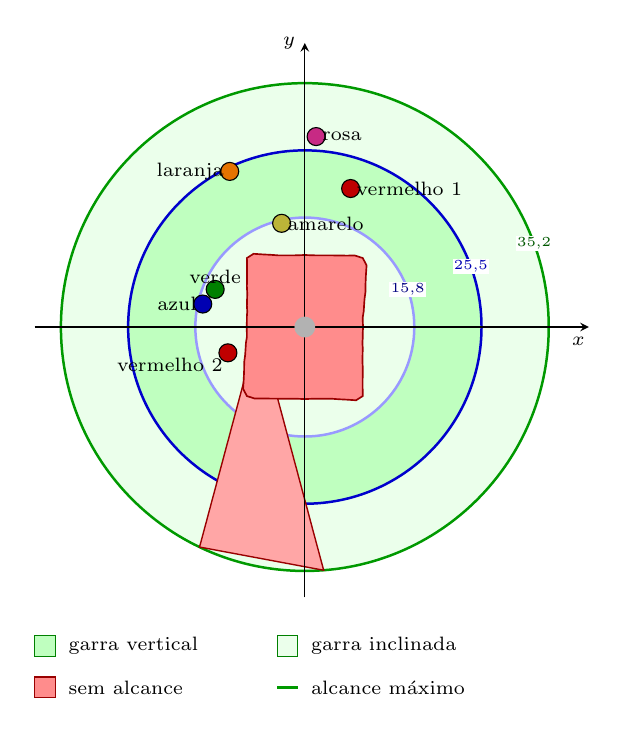
\begin{tikzpicture}[scale=0.088, >=stealth, every node/.style={font=\scriptsize}]
  \begin{scope}
    \clip (-40,-40) rectangle (40,40);
    \fill[green!8] (0,0) circle (35.2);
    \fill[green!25, even odd rule] (0,0) circle (25.5) (0,0) circle (15.8);
    \draw[green!60!black, line width=0.9pt] (0,0) circle (35.2);
    \draw[blue!80!black, line width=0.9pt] (0,0) circle (25.5);
    \draw[blue!40, line width=0.9pt] (0,0) circle (15.8);
    \filldraw[fill=red!35, draw=red!60!black, line width=0.5pt] (-7.63,-3.51) -- (-8.01,-4.92) -- (-8.35,-6.20) -- (-8.67,-7.40) -- (-8.98,-8.55) -- (-9.28,-9.67) -- (-9.57,-10.76) -- (-9.86,-11.83) -- (-10.14,-12.89) -- (-10.42,-13.93) -- (-10.70,-14.97) -- (-10.97,-16.00) -- (-11.25,-17.02) -- (-11.52,-18.03) -- (-11.79,-19.05) -- (-12.06,-20.05) -- (-12.33,-21.06) -- (-12.60,-22.06) -- (-12.86,-23.05) -- (-13.13,-24.05) -- (-13.40,-25.04) -- (-13.66,-26.03) -- (-13.93,-27.02) -- (-14.19,-28.01) -- (-14.46,-29.00) -- (-14.72,-29.98) -- (-14.98,-30.96) -- (-15.20,-31.75) -- (2.72,-35.10) -- (2.51,-34.31) -- (2.24,-33.32) -- (1.98,-32.34) -- (1.71,-31.35) -- (1.45,-30.37) -- (1.18,-29.38) -- (0.92,-28.39) -- (0.65,-27.39) -- (0.39,-26.40) -- (0.12,-25.40) -- (-0.15,-24.40) -- (-0.42,-23.40) -- (-0.69,-22.39) -- (-0.96,-21.38) -- (-1.23,-20.36) -- (-1.51,-19.34) -- (-1.78,-18.31) -- (-2.06,-17.28) -- (-2.34,-16.23) -- (-2.62,-15.18) -- (-2.91,-14.10) -- (-3.20,-13.01) -- (-3.50,-11.90) -- (-3.81,-10.74) -- (-4.13,-9.54) -- (-4.47,-8.27) -- (-4.85,-6.86) -- cycle;
    \filldraw[fill=red!45, draw=red!60!black, line width=0.6pt] (8.40,0.00) -- (8.37,0.73) -- (8.37,1.48) -- (8.50,2.28) -- (8.55,3.11) -- (8.61,4.01) -- (8.75,5.05) -- (8.76,6.14) -- (8.81,7.39) -- (8.91,8.91) -- (8.36,9.96) -- (7.23,10.32) -- (5.95,10.31) -- (4.82,10.33) -- (3.76,10.34) -- (2.77,10.34) -- (1.82,10.34) -- (0.91,10.36) -- (0.00,10.40) -- (-0.91,10.36) -- (-1.82,10.34) -- (-2.77,10.34) -- (-3.76,10.34) -- (-4.86,10.42) -- (-6.05,10.48) -- (-7.40,10.57) -- (-8.36,9.96) -- (-8.34,8.34) -- (-8.35,7.01) -- (-8.36,5.85) -- (-8.31,4.80) -- (-8.34,3.89) -- (-8.36,3.04) -- (-8.31,2.23) -- (-8.37,1.48) -- (-8.37,0.73) -- (-8.40,0.00) -- (-8.37,-0.73) -- (-8.37,-1.48) -- (-8.50,-2.28) -- (-8.55,-3.11) -- (-8.61,-4.01) -- (-8.75,-5.05) -- (-8.76,-6.14) -- (-8.81,-7.39) -- (-8.91,-8.91) -- (-8.36,-9.96) -- (-7.23,-10.32) -- (-5.95,-10.31) -- (-4.82,-10.33) -- (-3.76,-10.34) -- (-2.77,-10.34) -- (-1.82,-10.34) -- (-0.91,-10.36) -- (-0.00,-10.40) -- (0.91,-10.36) -- (1.82,-10.34) -- (2.77,-10.34) -- (3.76,-10.34) -- (4.86,-10.42) -- (6.05,-10.48) -- (7.40,-10.57) -- (8.36,-9.96) -- (8.34,-8.34) -- (8.35,-7.01) -- (8.36,-5.85) -- (8.31,-4.80) -- (8.34,-3.89) -- (8.36,-3.04) -- (8.31,-2.23) -- (8.37,-1.48) -- (8.37,-0.73) -- cycle;
  \end{scope}
  % eixos
  \draw[->, thin] (-39,0) -- (41,0) node[below left=0pt and -2pt] {$x$};
  \draw[->, thin] (0,-39) -- (0,41) node[left] {$y$};
  \fill[gray!60] (0,0) circle (1.5);
  % raios
  \node[blue!50!black, fill=white, inner sep=0.5pt, font=\tiny] at (20:15.8) {15,8};
  \node[blue!70!black, fill=white, inner sep=0.5pt, font=\tiny] at (20:25.5) {25,5};
  \node[green!35!black, fill=white, inner sep=0.5pt, font=\tiny] at (20:35.2) {35,2};
  % peças alcançadas
  \foreach \x/\y/\c/\n/\p in {
      6.61/19.99/red!75!black/vermelho 1/right,
      -11.10/-3.72/red!75!black/vermelho 2/below left,
      -10.84/22.46/orange!90!black/laranja/left,
      -3.35/14.97/yellow!70!black/amarelo/right,
      -12.94/5.43/green!50!black/verde/above,
      -14.73/3.32/blue!70!black/azul/left,
      1.63/27.49/magenta!80!black/rosa/right} {
    \filldraw[fill=\c, draw=black, thin] (\x,\y) circle (1.3);
    \node[\p=1pt, inner sep=1pt] at (\x,\y) {\n};
  }
  % legenda
  \begin{scope}[shift={(-39,-45)}]
    \filldraw[fill=green!25, draw=green!50!black] (0,-2.5) rectangle (3,0.5);
    \node[right] at (3.5,-1) {garra vertical};
    \filldraw[fill=green!8, draw=green!50!black] (35,-2.5) rectangle (38,0.5);
    \node[right] at (38.5,-1) {garra inclinada};
    \filldraw[fill=red!45, draw=red!60!black] (0,-8.5) rectangle (3,-5.5);
    \node[right] at (3.5,-7) {sem alcance};
    \draw[green!60!black, line width=0.9pt] (35,-7) -- (38,-7);
    \node[right] at (38.5,-7) {alcance máximo};
  \end{scope}
\end{tikzpicture}
    \caption{Peças da demonstração vistas de cima, no referencial da base (cm), com os limites de alcance.}
    \label{fig:mapa_alvos}
  \end{minipage}\hfill
  \begin{minipage}[b]{0.48\textwidth}
    \centering
    % Erros de modelo e de alcance, ordenados pela distância ao eixo da base (precisa de \usepackage{pgfplots})
% Feita para meia largura de página (dentro de uma minipage de 0,48\textwidth), sem \resizebox
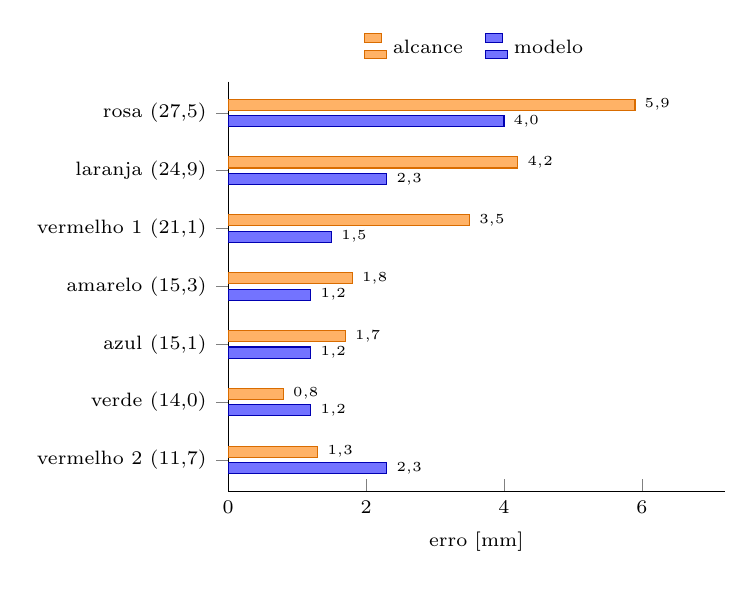
\begin{tikzpicture}
  \begin{axis}[xbar, bar width=4pt, scale only axis, width=0.52\linewidth, height=5.2cm,
      xmin=0, xmax=7.2, xlabel={erro [mm]},
      symbolic y coords={rosa, laranja, vermelho 1, amarelo, azul, verde, vermelho 2},
      ytick=data,
      yticklabels={{rosa (27,5)}, {laranja (24,9)}, {vermelho 1 (21,1)}, {amarelo (15,3)}, {azul (15,1)}, {verde (14,0)}, {vermelho 2 (11,7)}},
      y dir=reverse, enlarge y limits=0.09,
      tick label style={font=\scriptsize}, label style={font=\scriptsize},
      nodes near coords, every node near coord/.append style={font=\tiny},
      /pgf/number format/use comma, /pgf/number format/fixed, /pgf/number format/precision=1,
      /pgf/number format/fixed zerofill,
      legend style={at={(0.5,1.03)}, anchor=south, font=\scriptsize, draw=none, fill=none, legend columns=2, /tikz/every even column/.append style={column sep=6pt}},
      reverse legend,
      legend cell align=left,
      axis lines*=left, xtick={0,2,4,6}, xticklabels={0,2,4,6}]
    \addplot[fill=blue!55, draw=blue!70!black] coordinates
      {(4.0,rosa) (2.3,laranja) (1.5,vermelho 1) (1.2,amarelo) (1.2,azul) (1.2,verde) (2.3,vermelho 2)};
    \addplot[fill=orange!60, draw=orange!85!black] coordinates
      {(5.9,rosa) (4.2,laranja) (3.5,vermelho 1) (1.8,amarelo) (1.7,azul) (0.8,verde) (1.3,vermelho 2)};
    \legend{modelo, alcance}
  \end{axis}
\end{tikzpicture}
    \caption{Erros de modelo e de alcance em cada peça.}
    \label{fig:erros}
  \end{minipage}
\end{figure}

Nos sete alvos alcançáveis, a garra chegou a menos de 6~mm do ponto pedido e as juntas ficaram a menos de $1{,}6^\circ$ dos ângulos calculados. A altura $z = -10$~mm no referencial da base corresponde a 20~mm acima da mesa. Quatro peças, a 39--41~cm do eixo da base, foram declaradas inalcançáveis pela cinemática inversa antes de o braço se mover. O erro de alcance cresce com a distância ao eixo da base, sendo máximo no alvo mais afastado (rosa, a 27~cm), o que é compatível com o braço a descair com o próprio peso quando está mais esticado.
\subsection{Exemplo de execução}
\label{sec:exemplo_execucao}

Para ilustrar o movimento \textit{move end-effector to target position}, apresenta-se uma execução completa no CoppeliaSim, na qual o manipulador apanha um cubo vermelho, detetado pela câmara na posição $(X, Y, Z) = (0{,}225;\ 0{,}149;\ 0{,}010)$~m do referencial do mundo, e o leva até ao alvo verde. As posições são convertidas para o referencial da base através da função \texttt{world\_to\_base}, e a função \texttt{plan\_vertical} escolhe, antes de o braço se mover, a inclinação da garra para cada descida.

O cubo encontra-se a 30~cm do eixo da base, fora da zona em que a garra pode descer na vertical (Figura~\ref{fig:mapa_alvos}), pelo que é apanhado com uma inclinação de $70^\circ$. O alvo verde, mais próximo da base, permite pousar o cubo com uma inclinação de $95^\circ$.

A sequência, apresentada na Figura~\ref{fig:execucao}, é a seguinte:
\begin{enumerate}
    \item o manipulador parte da pose inicial (Figura~\ref{fig:execucao}a);
    \item a função \texttt{move\_joints} leva a garra até à posição de aproximação, por cima do cubo, e a função \texttt{move\_linear} desce até ele, que é agarrado (Figura~\ref{fig:execucao}b);
    \item a garra sobe, desloca-se até por cima do alvo verde e desce até à posição de pouso, onde o cubo é largado (Figura~\ref{fig:execucao}c);
    \item a garra sobe e a função \texttt{go\_home} leva o manipulador de volta à pose inicial (Figura~\ref{fig:execucao}d).
\end{enumerate}

\begin{figure}[H]
  \centering
  \begin{minipage}[b]{0.48\textwidth}
    \centering
    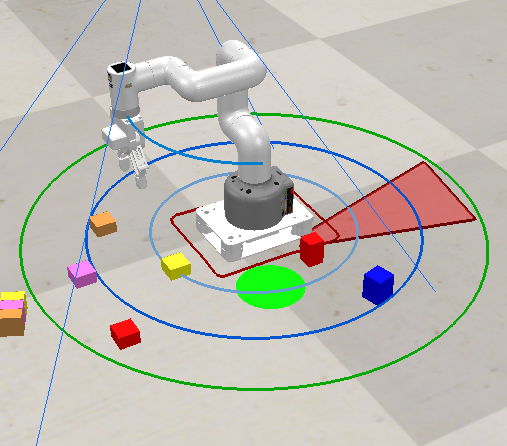
\includegraphics[width=\linewidth]{img/exec_1.png}\\[2pt]
    {\footnotesize (a) pose inicial}
  \end{minipage}\hfill
  \begin{minipage}[b]{0.48\textwidth}
    \centering
    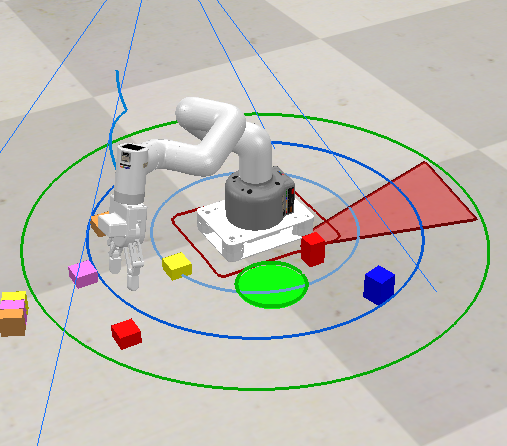
\includegraphics[width=\linewidth]{img/exec_2.png}\\[2pt]
    {\footnotesize (b) aproximação, por cima do cubo}
  \end{minipage}

  \vspace{6pt}
  \begin{minipage}[b]{0.48\textwidth}
    \centering
    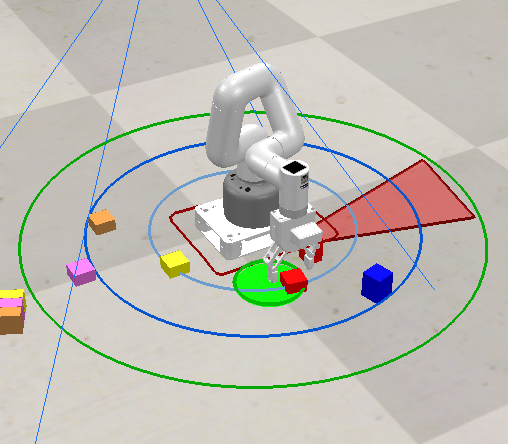
\includegraphics[width=\linewidth]{img/exec_3.png}\\[2pt]
    {\footnotesize (c) no alvo, a pousar o cubo}
  \end{minipage}\hfill
  \begin{minipage}[b]{0.48\textwidth}
    \centering
    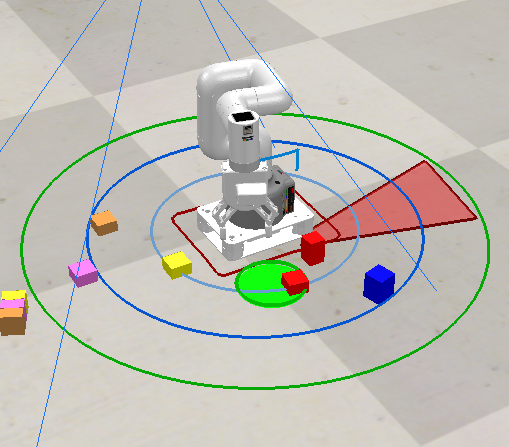
\includegraphics[width=\linewidth]{img/exec_4.png}\\[2pt]
    {\footnotesize (d) regresso à pose inicial}
  \end{minipage}
  \caption{Execução no CoppeliaSim: o cubo vermelho é levado até ao alvo verde. Na mesa estão desenhadas as zonas de alcance da Figura~\ref{fig:mapa_alvos}.}
  \label{fig:execucao}
\end{figure}

O Código~\ref{lst:execucao} apresenta a informação escrita pelo programa durante esta execução.

\begin{lstlisting}[basicstyle=\ttfamily\scriptsize, frame=single, breaklines=true,
                   caption={Saída do programa durante a execução da Figura~\ref{fig:execucao}.},
                   label={lst:execucao}]
--- tarefa 1 de 4 ---
pick_and_place: objeto no mundo [0.225 0.149 0.010], a 30 cm do eixo da base
pick_and_place: apanhar com a garra a 70 graus (J1 roda 38 graus), pousar a 95 graus (J1 roda 58 graus)
check_place: peça no sítio (red, 0.0 mm: não corrijo abaixo de 3 mm)
check_place: pilha deslocada 34.1 mm (green) -> [-0.021 0.177] em vez de [-0.000 0.150]
pick_and_place: concluído
Simulation time: 73.20 [s]
\end{lstlisting}

Antes de pousar o cubo, a câmara confirma a posição do destino. Nesta execução, o alvo verde foi detetado a 34,1~mm da posição esperada, e o ponto de pouso foi corrigido para a nova posição antes da descida. O movimento completo demorou 73,2~s de tempo de simulação. Os erros de posicionamento em diferentes posições alvo são apresentados na Tabela~\ref{tab:demo_sim}.
\section{Discussão}
\label{sec:disc}

\subsection{Validação do modelo}
 
O erro do modelo compara a posição calculada pela cinemática direta, com as juntas lidas no simulador, com a posição real do centro de preensão. Ficou entre 1,2 e 4,0~mm nos alvos testados, abaixo da tolerância de 5~mm, o que valida em conjunto a função \texttt{direct\_kin}, a conversão \texttt{world\_to\_base} e os comprimentos dos elos medidos no cenário. As diferenças que restam são pequenas e podem vir de os comprimentos medidos não coincidirem exatamente com a geometria do modelo do robô no CoppeliaSim e de o centro de preensão ser definido a partir de um ponto do modelo. Este erro não depende do movimento, pois só compara dois cálculos da mesma pose, e por isso mede a qualidade do modelo e não a do controlo.
 
\subsection{Erro de alcance e erro nas juntas}
 
O erro de alcance compara o ponto pedido com a posição real da garra, pelo que mistura dois efeitos: o erro do modelo e o facto de as juntas não chegarem exatamente aos ângulos pedidos. O erro nas juntas isola o segundo. Se o erro de alcance for semelhante ao erro do modelo e o erro nas juntas for pequeno, o movimento atinge o ponto pedido e o erro restante vem do modelo. Se o erro de alcance for maior, a diferença vem de as juntas ficarem ainda a caminho ou abaixo do ângulo pedido, por exemplo por efeito da gravidade ou do tempo de estabilização, de 2~s, ser curto para o movimento em causa.
\subsection{Alcance e inclinação da garra}
 
A cinemática inversa tenta primeiro a inclinação preferida, com a garra na vertical, e só se esta falhar inclina a garra. Com a implementação que usámos, para alvos a poucos centímetros da mesa, o alcance horizontal é de cerca de 27--28~cm do eixo da base com a garra na vertical e passa a cerca de 36--37~cm quando se permite inclinar a garra até $30^\circ$ da horizontal. Os alvos mais afastados da base são, por isso, os que exigem inclinar a garra, e são também os que deixam o braço quase esticado, onde pequenos erros nas juntas se traduzem em erros maiores de posição. Por outro lado, um alvo demasiado perto do eixo da base pode ser inalcançável, porque o desvio lateral $L_5$ impede a garra de chegar ao eixo de J1.
 
\subsection{Limitações}
 
O movimento \texttt{move\_joints} interpola as juntas, e não a posição da garra, pelo que a trajetória do \textit{end-effector} entre dois pontos não é uma reta; passa pela pose inicial para evitar a mesa, mas não é uma trajetória planeada no espaço cartesiano. Quando é preciso um movimento em linha reta, usa-se \texttt{move\_linear}, que resolve a cinemática inversa a cada passo. Além disso, os resultados são de simulação e usam as posições reais dos objetos, que só o simulador conhece, apenas para definir os alvos e medir os erros; no braço real, os alvos viriam da câmara e não existiria o erro do modelo medido desta forma.
 

\setcounter{table}{0}
\setcounter{figure}{0}


\chapter{Conclusão}
\label{ch:conclusao}

Neste trabalho, foi desenvolvida e implementada a cinemática do manipulador robótico myCobot~280, desde a formulação matemática dos modelos de cinemática direta e inversa até à demonstração do movimento do centro de preensão da garra para diferentes posições alvo, utilizando o MATLAB em comunicação com o CoppeliaSim.

Os objetivos inicialmente definidos foram cumpridos, tendo sido deduzidos os modelos cinemáticos, realizada a sua implementação em MATLAB e estabelecida a integração com o ambiente de simulação. A validação foi efetuada através de exemplos numéricos e de testes de posicionamento do manipulador.

\section*{Formulação}

A cinemática direta foi desenvolvida através de uma abordagem geométrica, baseada na decomposição do manipulador em dois planos.

No plano lateral, a posição do centro de preensão é determinada a partir das projeções dos elos, utilizando os ângulos absolutos associados às juntas J2, J3 e J4, bem como a inclinação da garra. No plano horizontal, a rotação da junta J1 e o desvio lateral $L_5$ permitem determinar as coordenadas cartesianas $(x,y,z)$ relativamente ao referencial da base.

A cinemática inversa foi formulada recorrendo à mesma decomposição geométrica, mas seguindo a ordem inversa dos cálculos.

Inicialmente, no plano horizontal, são determinadas a orientação da base, $q_1$, e a distância frontal $d$. Posteriormente, no plano lateral, fixa-se uma inclinação para a garra e reduz-se o problema a um manipulador planar de dois graus de liberdade, resolvido através da lei dos cossenos. Esta resolução permite determinar os ângulos das juntas J2 e J3, sendo o ângulo de J4 calculado a partir da orientação pretendida para a garra.

Para uma inclinação fixa, a resolução é analítica, sendo verificadas as condições de alcançabilidade e os limites articulares. Por defeito, é utilizada a configuração com o cotovelo para cima.

Quando não existe uma solução válida para a inclinação preferencial de $90^\circ$, o algoritmo procura inclinações alternativas, realizando posteriormente um refinamento por bisseção para encontrar uma orientação próxima da inicialmente pretendida.

Esta abordagem permitiu alcançar posições que seriam inacessíveis com a garra orientada verticalmente para baixo. No segundo exemplo analisado, correspondente a um alvo situado a aproximadamente $30$ cm do eixo da base, foi necessário ajustar a inclinação da garra para cerca de $82{,}27^\circ$.

Em ambos os exemplos, a aplicação da cinemática direta aos ângulos obtidos pela cinemática inversa permitiu recuperar as posições pretendidas dentro da precisão numérica considerada, confirmando a consistência matemática dos modelos desenvolvidos.

\section*{Implementação e resultados}

Os modelos cinemáticos foram implementados em MATLAB através das funções \texttt{direct\_kin} e \texttt{inverse\_kin}, sendo posteriormente integrados com as funções responsáveis pela execução dos movimentos do manipulador.

A função \texttt{move\_joints} permite executar movimentos suaves no espaço das juntas, enquanto a função \texttt{move\_linear} é utilizada para realizar trajetórias aproximadamente retilíneas no espaço cartesiano.

Para movimentos verticais, a função \texttt{plan\_vertical} permite selecionar uma inclinação fixa da garra que seja válida ao longo de toda a trajetória. Por sua vez, a função \texttt{go\_home} permite regressar à configuração inicial, realizando previamente uma subida de segurança quando necessário.

A comunicação entre o MATLAB e o CoppeliaSim foi estabelecida em modo síncrono, permitindo coordenar o envio dos comandos articulares com a evolução da simulação. As funções de movimento utilizam as leituras das juntas para acompanhar a execução e avaliar a posição do centro de preensão.

Na demonstração realizada no simulador, o manipulador foi deslocado até diferentes peças distribuídas sobre a mesa.

Nos sete alvos alcançados, o erro de posicionamento foi inferior a $6$ mm, com um valor máximo de $5{,}9$ mm. As diferenças articulares máximas registadas variaram entre $0{,}4^\circ$ e $1{,}6^\circ$.

O erro do modelo, calculado através da comparação entre a posição fornecida pela cinemática direta e a posição do centro de preensão obtida no CoppeliaSim, situou-se entre $1{,}2$ mm e $4{,}1$ mm, permanecendo abaixo da tolerância de $5$ mm considerada no diagnóstico.

Estes resultados demonstram uma boa correspondência entre o modelo geométrico implementado e o posicionamento do manipulador no ambiente de simulação.

Os testes de alcance também evidenciaram a importância da inclinação da garra. Para alvos situados a poucos centímetros da superfície da mesa, verificou-se um alcance horizontal aproximado de $27$ a $28$ cm relativamente ao eixo da base, mantendo a garra vertical.

Ao permitir a alteração da inclinação da garra, considerando valores até $\psi=30^\circ$, o alcance aumentou para aproximadamente $36$ a $37$ cm nas condições testadas.

Por outro lado, quatro posições situadas a cerca de $39$ a $41$ cm do eixo da base foram rejeitadas pela cinemática inversa antes da execução do movimento, por não terem sido encontradas configurações válidas segundo as restrições implementadas.

Deste modo, os resultados demonstraram não apenas a capacidade de posicionamento do manipulador, mas também a importância da verificação da alcançabilidade antes da execução dos movimentos.

\section*{Limitações}

Apesar dos resultados obtidos, foram identificadas algumas limitações na abordagem desenvolvida.

Em primeiro lugar, os erros de posicionamento podem ser influenciados pelas diferenças entre o modelo geométrico e o modelo utilizado no simulador, bem como pelos desvios entre os ângulos articulares pretendidos e os efetivamente atingidos.

O maior erro de alcance foi registado na peça rosa, uma das mais afastadas da base, sendo compatível com uma maior dificuldade de posicionamento quando o manipulador apresenta uma configuração mais estendida.

Nestas condições, pequenas diferenças articulares podem provocar desvios mais significativos no centro de preensão. Os efeitos da gravidade e o tempo de estabilização também podem contribuir para estas diferenças, embora não tenha sido possível determinar isoladamente a sua influência.

Outra limitação está relacionada com a estratégia de movimento. A interpolação realizada pela função \texttt{move\_joints} não garante uma trajetória retilínea do centro de preensão, sendo necessário recorrer à função \texttt{move\_linear} quando se pretende seguir uma trajetória cartesiana.

Além disso, a resolução da cinemática inversa considera a junta J5 fixa a $0^\circ$ e privilegia, por defeito, a configuração com o cotovelo para cima. Estas escolhas simplificam a implementação, mas limitam o conjunto de configurações articulares exploradas.

Por fim, os resultados apresentados foram obtidos em ambiente de simulação. Embora o CoppeliaSim permita avaliar os algoritmos em condições controladas, a sua utilização não substitui os testes num manipulador físico.

A identificação e localização dos objetos num sistema real também introduziriam fontes adicionais de erro, associadas ao sistema de visão e à calibração entre os diferentes referenciais.

\section*{Trabalho futuro}

Como trabalho futuro, pretende-se adaptar a implementação desenvolvida para a utilização com o manipulador físico myCobot~280, aproveitando os modelos cinemáticos e as funções de movimento já implementados.

Uma das primeiras etapas consistirá na calibração de uma câmara real, de forma a identificar a posição das peças sobre a mesa e converter corretamente as coordenadas detetadas para o referencial da base do manipulador.

Será também necessário adaptar a interface de comunicação utilizada em MATLAB para permitir o envio de comandos diretamente ao robô físico, substituindo a comunicação com o ambiente de simulação.

Outra etapa importante será a calibração das juntas, incluindo a verificação dos respetivos pontos de referência e a avaliação de possíveis diferenças entre o modelo geométrico e o comportamento real do manipulador.

Deverão ainda ser estudadas estratégias para compensar os efeitos da gravidade, as folgas mecânicas e os erros de posicionamento, particularmente em configurações mais estendidas.

Por fim, será importante reforçar as condições de segurança durante a execução dos movimentos, através da limitação das velocidades e das forças aplicadas, bem como da verificação de possíveis colisões com os objetos e com o ambiente de trabalho.

Estas melhorias permitirão evoluir da validação em simulação para a implementação experimental de um sistema de manipulação robótica, integrando cinemática, planeamento de movimentos e visão artificial.

\setcounter{table}{0}
\setcounter{figure}{0}

% Precisa de \usepackage{url} (ou hyperref) no preâmbulo
\begin{thebibliography}{9}

\bibitem{bicho_2dof}
E.~Bicho Erlhagen, \textit{Planar Robot Arms with 2 DOF: forward and inverse kinematics} (abordagem geométrica), diapositivos da UC Sistemas Autónomos Inteligentes, Universidade do Minho, 2024.

\bibitem{bicho_3dof}
E.~Bicho Erlhagen, \textit{Planar Robot Arms with 3 DOF (RRR): forward and inverse kinematics \& redundancy problem}, diapositivos da UC Sistemas Autónomos Inteligentes, Universidade do Minho, 2023.

\bibitem{louro_coppelia}
L.~Louro, \textit{CoppeliaSim: Simuladores de robótica}, diapositivos da UC Sistemas Autónomos Inteligentes 2026/2027, Universidade do Minho, set. 2026.

\bibitem{louro_matlab}
L.~Louro, \textit{CoppeliaSim: Simulador de robótica para SAI e SDNL}, diapositivos da UC Sistemas Autónomos Inteligentes 2026/2027, Universidade do Minho, out. 2026.

\bibitem{louro_codigo}
L.~Louro e E.~Bicho, \textit{Windows\_zeromq\_mycobot}: interface MATLAB--CoppeliaSim para o myCobot~280 (\texttt{main\_program.m}, \texttt{mycobot\_interface.m}, \texttt{simulator\_interface.m}) e cenário \texttt{mycobot280\_vision.ttt}, código fornecido na UC Sistemas Autónomos Inteligentes, Universidade do Minho, 2026.

\bibitem{coppelia_zmq}
Coppelia Robotics AG, \textit{ZeroMQ remote API client para MATLAB} (\texttt{RemoteAPIClient.m}, \texttt{cbor.m}), com a biblioteca JeroMQ~0.5.2, 2022.

\bibitem{elephant}
Elephant Robotics, \textit{myCobot 280: documentação}, \url{https://docs.elephantrobotics.com}.

\bibitem{coppelia_manual}
Coppelia Robotics, \textit{CoppeliaSim User Manual: ZeroMQ remote API}, \url{https://manual.coppeliarobotics.com}.

\bibitem{matlab}
The MathWorks, \textit{MATLAB Documentation}, \url{https://www.mathworks.com/help/matlab/}.

\end{thebibliography}
\setcounter{table}{0}
\setcounter{figure}{0}
%\input{tex/Chap/INTRO} % Introduction
%\input{kalman_equations}
%\input{ANALYSIS} % Analysis of the problem
%\input{DESIGN} % Algorithms design and Workflow
%\input{EX1} % Matlab implementation
%\input{tex/Chap/NEURON-NO-SELF-EXCITATION} % EX1
%\input{tex/Chap/NEURON-SELF-EXCITATION} % EX2
%\input{tex/Chap/TWO-NEURONS} % EX3
%\input{tex/Chap/TARGET-SELECTION} % EX4
%\input{TESTS} % Testing
%\input{tex/Chap/CONCLUSION} % Conclusions and Future Work
%
% -------------- BIBLIO ---------------------
%\bookmarksetup{startatroot} % Ends last part.
%\bibliographystyle{unsrtnat}
%\renewcommand{\bibname}{Referências} 
%\bibliography{bib/dissert}


\end{document}
